\documentclass[a4paper,12pt,twoside]{article}
\usepackage[T1]{fontenc}
\usepackage[utf8]{inputenc}
\usepackage{lmodern}
\usepackage{url,csquotes}
\usepackage[hidelinks,hyperfootnotes=false]{hyperref}
\usepackage[titlepage,pagenumber]{polytechnique}
\usepackage{float}

\title{MAP-536 - Python for Data Science}
\subtitle{Final Project - Air data prediction}
\author{Leonardo \textsc{Natale} \& Guillaume \textsc{Le Fur}}
\logo{scikit_learn.jpeg}

\begin{document}

\maketitle

\section{External Data and Data Preprocessing}

\subsection{Getting External Data}
The original data consists of:
\begin{itemize}
	\item the date of departure
	\item the departure and arrival airport
	\item the mean and standard deviation of the number of weeks of the reservations made before the departure date
    \item a field called log\_PAX which is related to the number of passengers (the actual number were changed for privacy reasons)
\end{itemize}
We have added the following data:
\begin{itemize}
	\item Daily Jet Fuel Price
	\item Airport Location (geographical coordinates)
	\item Departure and Arrival GDP
	\item Monthly flow of passengers in the US between airports.
	\item Daily Weather Data
	\item US Holiday Calendar
\end{itemize}

\subsection{Feature Engineering}

We were able to add the following extra features, by using the data described above:
\begin{itemize}
	\item Number of days to the closest holiday.
	\item Distance in kilometers between departure and arrival airport.
	\item Airport Dimension
	\item Monthly log\_PAX per airport, both arrival and departure.
\end{itemize}


\section{Structure}
(Adjust the size and position, maybe explanation at the right)
\begin{figure}[H]
	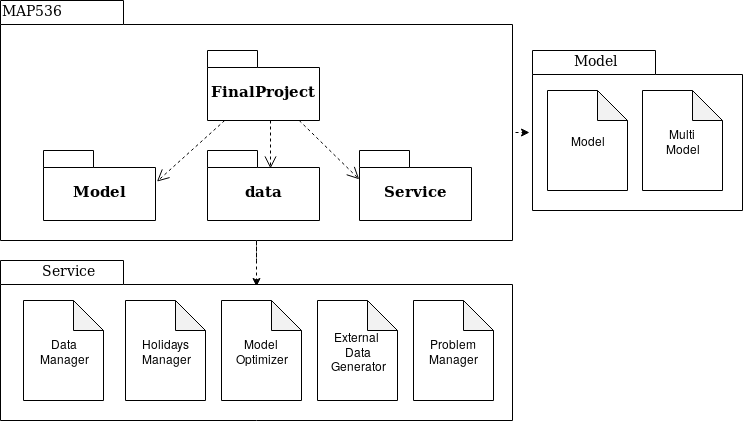
\includegraphics[width=100mm,scale=0.5]{UML.png}
\end{figure}

\section{Models and Tuning}
\subsection{Models}
Add a table with comparison between different models.
\begin{center}
	\begin{tabular}{||c || c c c||} 
		\hline
			 & Train RMSE & Test RMSE & Train time (s) \\ [0.5ex] 
		\hline\hline
		\textbf{Model1} & 6 & 87837 & 787 \\ 
		\hline
		\textbf{Model2} & 7 & 78 & 5415 \\
		\hline
		\textbf{Model3} & 545 & 778 & 7507 \\
		\hline
	\end{tabular}
\end{center}
Explain why we have chosen our model.

\subsection{Hyperparameters Tuning}
Our ModelOptimizer class is in charge of the optimization of the models by Grid Search and Randomized Search. It is composed by two methods:
\begin{itemize}
	\item grid\_search\_optimize runs a GridSearchCV with the given params and outputs the optimal value of the parameters for the model.
	\item random\_search\_optimize runs a a RandomSearchCV with the given params to which we associate the given distribution.
\end{itemize}

\section{Conclusion}
\subsection{Model Interpretability}
Feature importance graph and comments.
\subsection{Evaluation of Uncertainty in Predictions}
Talk about: 
\subsection{Final Comments and Possible Improvements}

\end{document}
